\documentclass[tikz,border=6pt]{standalone}
\usetikzlibrary{arrows.meta,positioning,calc}

% ---- tunable quantities -------------------------------------------------
\newcommand{\NodeW}{34mm}   % width of a knowledge-component box
\newcommand{\ColGap}{26mm}
\definecolor{ink}{HTML}{1A1A1A}
\definecolor{rule}{HTML}{9AA3AB}
\definecolor{edge}{HTML}{555555}
\definecolor{tint}{HTML}{F7E9E9}

\begin{document}
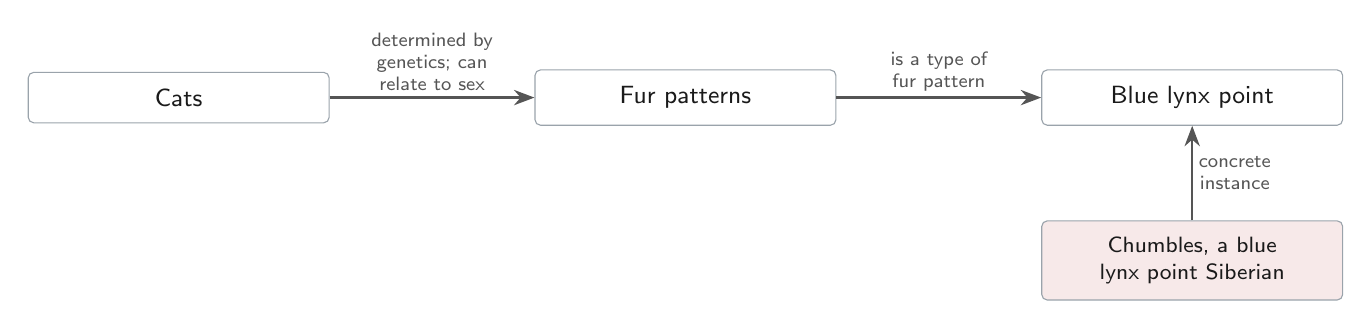
\begin{tikzpicture}[
  font=\sffamily\small,
  kc/.style={draw=rule, fill=white, rounded corners=2pt, text width=\NodeW,
             align=center, inner sep=6pt, text=ink},
  proof/.style={draw=rule, fill=tint, rounded corners=2pt, text width=\NodeW,
                align=center, inner sep=6pt, text=ink, font=\sffamily\footnotesize},
  rel/.style={-{Stealth[length=2.6mm]}, draw=edge, thick},
  lab/.style={font=\sffamily\scriptsize, text=edge, align=center,
              fill=white, inner sep=2pt}
]
% ---- components (drawing order: nodes, then relations, then labels) -----
\node[kc] (cats) {Cats};
\node[kc, right=\ColGap of cats] (fur) {Fur patterns};
\node[kc, right=\ColGap of fur] (blp) {Blue lynx point};
\node[proof, below=12mm of blp] (chum) {Chumbles, a blue lynx point Siberian};

% ---- relations ----------------------------------------------------------
\draw[rel] (cats) -- node[lab, midway, above] {determined by\\genetics; can\\relate to sex} (fur);
\draw[rel] (fur) -- node[lab, midway, above] {is a type of\\fur pattern} (blp);
\draw[rel] (chum) -- node[lab, midway, right] {concrete\\instance} (blp);
\end{tikzpicture}
\end{document}
